\documentclass[12pt,a4paper]{article}

% 使用中文宏包
\usepackage[UTF8]{ctex}
\usepackage{graphicx} %插入图片的宏包
\usepackage{float} %设置图片浮动位置的宏包
\usepackage[strings]{underscore}
\usepackage{times}
\usepackage{epsfig}
\usepackage{amsmath}
\usepackage{amssymb}
\usepackage{overpic}
\usepackage{listings}
\usepackage{color}
\usepackage{enumitem}
\setenumerate[1]{itemsep=0pt,partopsep=0pt,parsep=\parskip,topsep=5pt}
\setitemize[1]{itemsep=0pt,partopsep=0pt,parsep=\parskip,topsep=5pt}
\setdescription{itemsep=0pt,partopsep=0pt,parsep=\parskip,topsep=5pt}

\definecolor{mygreen}{rgb}{0,0.6,0}
\definecolor{mygray}{rgb}{0.5,0.5,0.5}
\definecolor{mymauve}{rgb}{0.58,0,0.82}
\lstset{ %
  backgroundcolor=\color{white},   % choose the background color
  basicstyle=\footnotesize,        % size of fonts used for the code
  breaklines=true,                 % automatic line breaking only at whitespace
  captionpos=b,                    % sets the caption-position to bottom
  commentstyle=\color{mygreen},    % comment style
  escapeinside={\%*}{*)},          % if you want to add LaTeX within your code
  keywordstyle=\color{blue},       % keyword style
  stringstyle=\color{mymauve},     % string literal style
}

\usepackage[pagebackref=true,breaklinks=true,letterpaper=true,colorlinks,bookmarks=false]{hyperref}


\def\httilde{\mbox{\tt\raisebox{-.5ex}{\symbol{126}}}}


\graphicspath{{figures/}}

\setcounter{page}{1}

\begin{document}


%%%%%%%%% TITLE

\title{论文阅读笔记:隐私}
\author{纳文琪}
\maketitle


\section{Big Privacy: Challenges and Opportunities of Privacy Study in the Age of Big Data\cite{yu2016big}}

\subsection{引言}
\paragraph{} 最近研究表明,在大数据时代简单地匿名化数据集已无法再抵御针对隐私的攻击。保护隐私最直接的办法就是移除数据集中的ID,然而,事实表明这并不奏效。本质上,一个ID表示的是被描述对象的一组特征,但是实际上,我们依靠一个人的多种特征而不是ID来识别这个人。
\paragraph{隐私研究的两个方面} 隐私研究集中在两个方面:内容隐私(content privary)和行为隐私(interaction privacy)。
	\subparagraph{内容隐私} 攻击者根据受害者的一些知识背景从匿名或加密的数据集中识别受害者身份。
	\subparagraph{行为隐私} 攻击者更关注受害者的行为。
\paragraph{} 现代隐私研究主要关注两个方面:数据聚类(data clustering)和隐私框架(privacy framework)。


\subsection{基础知识}
\paragraph{隐私参与者} 包括:数据生产者、使用者、管理者、攻击者。
\paragraph{数据操作} 包括:收集、清洗(anonymizing)、交换(communicating)。
\paragraph{数据属性的类型} 包括:
	\subparagraph{显示标识(explicit identifier)} 比如身份证号、特定学校里的学号等;
	\subparagraph{准标识(quasi-identifier)} 通过关联其他数据集就可以确定用户的属性,比如性别、年龄等。我们一般将一个记录里面的所有准标识字段称为“qid”。拥有相同qid的值的一组记录被称为一个等价类(equivalent class)。
	\subparagraph{敏感信息(sensitive information)} 用户希望保护的那部分数据;
	\subparagraph{其他} 用户的其他信息。

\subsection{隐私研究的成果} 
\subsubsection{数据聚类方面}
\paragraph{} 数据聚类方面的研究成果主要包括:k-anonymity、l-diversity、t-closeness等。
\paragraph{k-anonymity} 首先,为保护隐私,我们必须将数据的ID全部移除,这样才能避免特定用户被识别。然而即便所有ID被移除,攻击者还是有可能通过诸如链接外部数据库等方式,根据qid来识别用户。k-anonymity方法的基本原则是:确保含有相同qid组数据的记录在数据集中至少出现k次,也就是说,每个等价类至少有k个记录。这样就可以使得攻击者通过qid识别特定用户的概率变为$\frac{1}{k}$,当存在一个很大的k值的时候,会对用户的识别产生一个很大的信息损失,从而达到隐私保护的作用。k-anonymity方法主要是用于处理准标识字段上的隐私保护问题,但不能处理敏感数据。攻击者可能使用同质攻击(homogeneity attach)或背景知识攻击(backgroud knowledge attack)来破解。
\paragraph{l-diversity} l-diversity方法可以克服k-anonymity方法的缺点。它要求数据集“对每一个qid的值,确保敏感数据字段至少有l个不同的值”。为了实现它,我们需要增大(还是减小?)敏感信息字段的颗粒度或增加噪声。某些特殊的时候,l-diversity会起到反作用,他会释放更多的信息增益给攻击者。
\paragraph{t-closeness} 可以修复l-diversity的脆弱性。它的基本思想是:对于任何一个等价类,保证它的值的分布被限定在t范围内。

\subsubsection{隐私框架方面}
\paragraph{微分隐私(differential privacy)} 在了解用户背景知识的情况下,攻击者可能会通过多次进行统计查询来获得期望的信息。防范策略是:对两个差别很小的数据集进行查询,其结果差别也应该很小,这样就可以限制攻击者获得的信息增益。
\paragraph{微分可识别性(differential identifiability)}
\paragraph{成员隐私(membership privacy)} 

\subsection{隐私研究的学科}

\subsection{隐私研究的数学描述}
\paragraph{匿名系统} 是一个映射函数:$F = X \rightarrow Y$,$X = \left \{ X_1,X_2,...,X_n \right \}$是原始数据,$Y=\left \{ Y_1,Y_2,...,Y_m \right \}$是系统的输出,对于攻击者,其目的是建立一个映射:$G: Y \rightarrow \hat X$,尽可能地从输出还原原始数据。
\paragraph{隐私保护系统的两个目的} 被描述为utility和privacy,这也是匿名系统F的两个关键指标。
	\subparagraph{utility} 使用 distorion D来度量,抽象地表示为:
	\begin{equation}
		D=\lambda(X;Y)
	\end{equation}
	D有很多种度量方法,例如,可以使用均方来表示。
	\subparagraph{privacy} 使用 leakage L 来度量,抽象地表示为:
	\begin{equation}
		L=\lambda(X;\hat X)
	\end{equation}
	L通常使用互信息来度量,即:
	\begin{equation}
		L=I(X,\hat X)
	\end{equation}
	
\paragraph{} 给定两个阈值$D_0$和$L_0$,匿名系统可作为一个优化问题:
\begin{equation}
  \begin{split}
  	optimize F \\
	s.t. \ D &\leq D_0 \\
	L &\leq L_0
  \end{split}
\end{equation}


\subsection{隐私度量(Privacy Measurements)}
\paragraph{}隐私的度量至今都没有太清晰的方法。现有以下几种度量方法:

	\subsubsection{相对度量(Relative Measurement)}
	\paragraph{} 其思想是:首先给定一个标准(benchmark),再度量研究对象到此标准的距离。比较流行的距离计算方式是Kullback-Leibler距离(相对熵)。
	\paragraph{} KL距离是基于一阶统计的度量方法,而二阶方法可以度量得更加精确。

	\subsubsection{信息论度量(Information Theoretic Measurement)}
	\paragraph{} 对于一个投票系统,定义三个随机变量V、S、E,分别表示投票者所投的票、来自投票系统以外的信息、攻击者由投票系统中获得的信息。
	\paragraph{完美隐私(perfectly privacy)} 定义为:在S条件下,V和E独立。即:$p_{V|S}(v;s) = p_{V|S,E}(v;s,e)$。
	\paragraph{隐私损失总量(amount of privacy loss)} 定义为:
	\begin{equation}
		L = \max (H(V|S) - H(V|S,E))
	\end{equation}
	度量隐私可能纰漏的程度。
	
	\subsubsection{Unicity Measure}

\subsection{隐私数学模型}

	\subsubsection{k-anonymity 模型}
	\paragraph{} 定义数据表$T=\left \{ t_1, t_2,...,t_n \right \}$ 是数据行的集合,$A=\left \{ A_1, A_2,...,A_n \right \}$ 是数据的属性集,$t_i[A_j]$表示元组$t_i$的属性$A_j$的值,$C=\left \{ C_1,C_2,...,C_k \right \} \subseteq A $是子属性集。定义 $T[C] = \left \{ t[C_1],t[C_2],...,t[C_k] \right \}$是t在C上的映射,$QI$为所有准标识符的集合。
	\paragraph{} 我们说一个表T满足k-anonymity,如果它满足,对于每一个元组$t \in T $ 都存在$k-1$个其他的元组$t_{i_1},t_{i_2},...,t_{i{k-1}} \in T $使得 $t[C]=t_{i_1}[C]=t_{i_2}[C]=...=t_{i_{k-1}}[C], C \subseteq QI$。也就是说,任何一组具有相同属性值的准标识符在表中至少出现k次。
	\subsubsection{l-diversity 模型}
	\subsubsection{t-closeness 模型}
	\subsubsection{Differential Privacy 框架}


\section{k-anonymity: A model for protecting privacy \cite{k-anonymity}}

\subsection{背景}
\paragraph{} 人们希望大量数据用于研究和分析,但同时又保证不泄露隐私,即同时满足“数据利用(utility)”和“保护隐私(privacy)”两个要求。通常,人们在发布数据时,会将数据集的标识符(如姓名、身份证号等)删去,从而使得数据集中的个体(individual)不能够被攻击者“重新识别(re-identify)”。然后,在很多情况下,利用非标识符字段仍然可以重新识别出个体。例如,研究显示,87\%的美国人可以通过邮编、性别和生日被识别出来。k-anonymity提供了一种避免此问题的框架。

\subsection{定义}
\paragraph{纰漏(disclosure)}指的是数据明显地或通过推理被意外地泄露。
\paragraph{纰漏控制(disclosure control)} 的目的是去识别或限制发布数据中的纰漏,也就是说,确保发布数据具有充分的匿名性。
\paragraph{准标识符(Quasi-identifier)} 如果数据表中的一组属性,可以通过与外部属性连接重新识别数据表中的个体,则称这组属性为准标识符。
\paragraph{准标识符的形式化定义} 令U为数据个体的全集,$T(A_1,...,A_n)$为数据表,存在两个映射$f_c: U \rightarrow T$和$f_g: T \rightarrow U'$,其中$U' \subseteq U$。表T的准标识符$Q_T$是一个属性集$\left \{ A_1,...,A_j\right \} \subseteq \left \{ A_1,...,A_n \right \}$,满足 $\exists p_i \in U $使得 $f_g(f_c(pi)[Q_T]) = p_i$。

\subsection{模型}
\paragraph{k-anonymity} 有表T和它的准标识符$Q_T$,当且仅当$T[Q_T]$中的每一行在$T[Q_T]$中至少出现k次时,我们说T满足k-anonymity。
\begin{figure}[H]
	\centering
	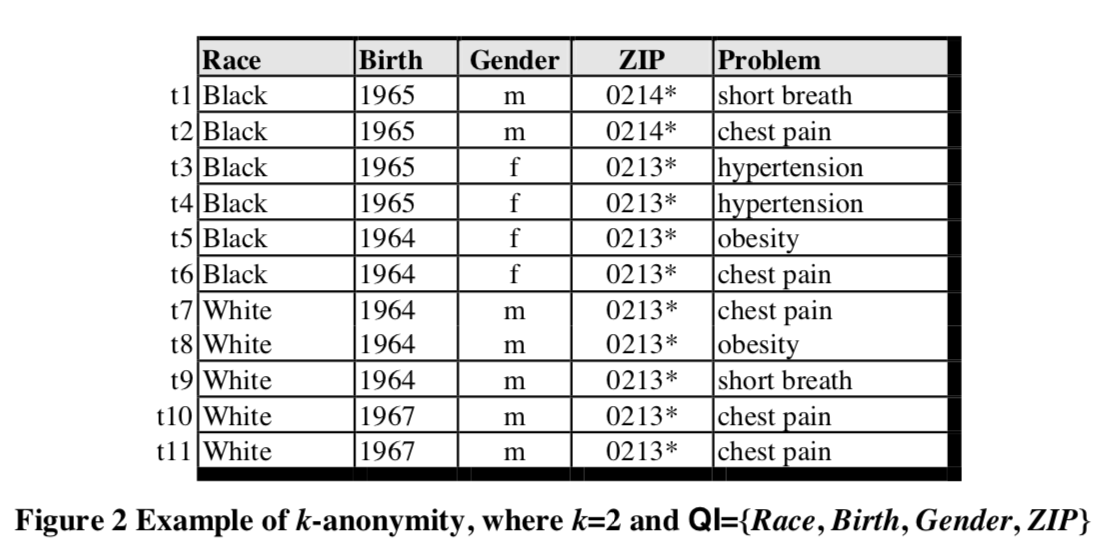
\includegraphics[width=0.7\textwidth]{../images/k-anonymity-example.png}
	\caption{}
	\label{}
\end{figure}

\subsection{攻击k-anonymity}
\paragraph{未排序匹配(Unsorted matching)攻击} 如果发布的表的数据的顺序固定,就可以根据这种固定顺序,关联多个发布的表来获取敏感信息。避免这种攻击很简单,只需要对数据进行乱序操作后再发布即可。
\paragraph{互补发布攻击(Complementary release attack)} 通常情况下,我们不会将所有发布的字段都列为准标识符,这样的话,如果同意数据表被发布了多个版本,攻击者就可能会通过关联多个发布的数据表来攻击k-anonymity。

\paragraph{时间攻击(Temporal attack)} 如果数据集是动态变化的,由于每个时间的数据表都可能不一样,而不同时间点之间的数据表没有规则限制,因此攻击者有可能通过关联两个不同时间点数据集来识别数据表中的个体,从而实现对k-anonymity的攻击。两个不同时间点的数据表就与上面所讲的两个不同版本的数据集类似。

\section{Protecting respondents identities in microdata release \cite{samarati2001}}
\paragraph{} 本文提出了一种实现k-anonymity的泛化算法。

\subsection{泛化数据(Generalizing data)}
\subsubsection{泛化关系(Generalization relationships)}
\paragraph{泛化关系} 是关于全体值域的集合Dom上的一个偏序,记作$ \leq_D $。它满足两个条件:
\begin{itemize}
	\item $ \vee D_i,D_j,D_z \in Dom  : D_i \leq_D D_j,  D_i \leq_D D_z \Rightarrow D_j \leq_D D_z \vee D_z \leq_D D_j $ (每个$D_i$最多只有一个直接泛化域)
	\item 域中的所有值最终都被泛化到一个单一值(单一最大值)
\end{itemize}
\paragraph{域泛化结构(domain generalization hierarchy, $DGH_D$} 由泛化关系得到的一个全序结构。
\paragraph{值泛化关系(value generalization relationships)} 是与DGR类似的,关于某个值域D下的所有值的一个偏序,记作$ \leq_V$
\paragraph{值泛化结构(value generalization hierarchy, $VGH_D$)} 与$DGH_D$类似,可以用树来表示,其叶子节点就是域D中的值。
\paragraph{} 值泛化关系和值泛化结构可以看做是域泛化关系和域泛化结构更低层次的抽象。其示例如图 \ref{dgh-vgh} 。
\begin{figure}[H]
	\centering
	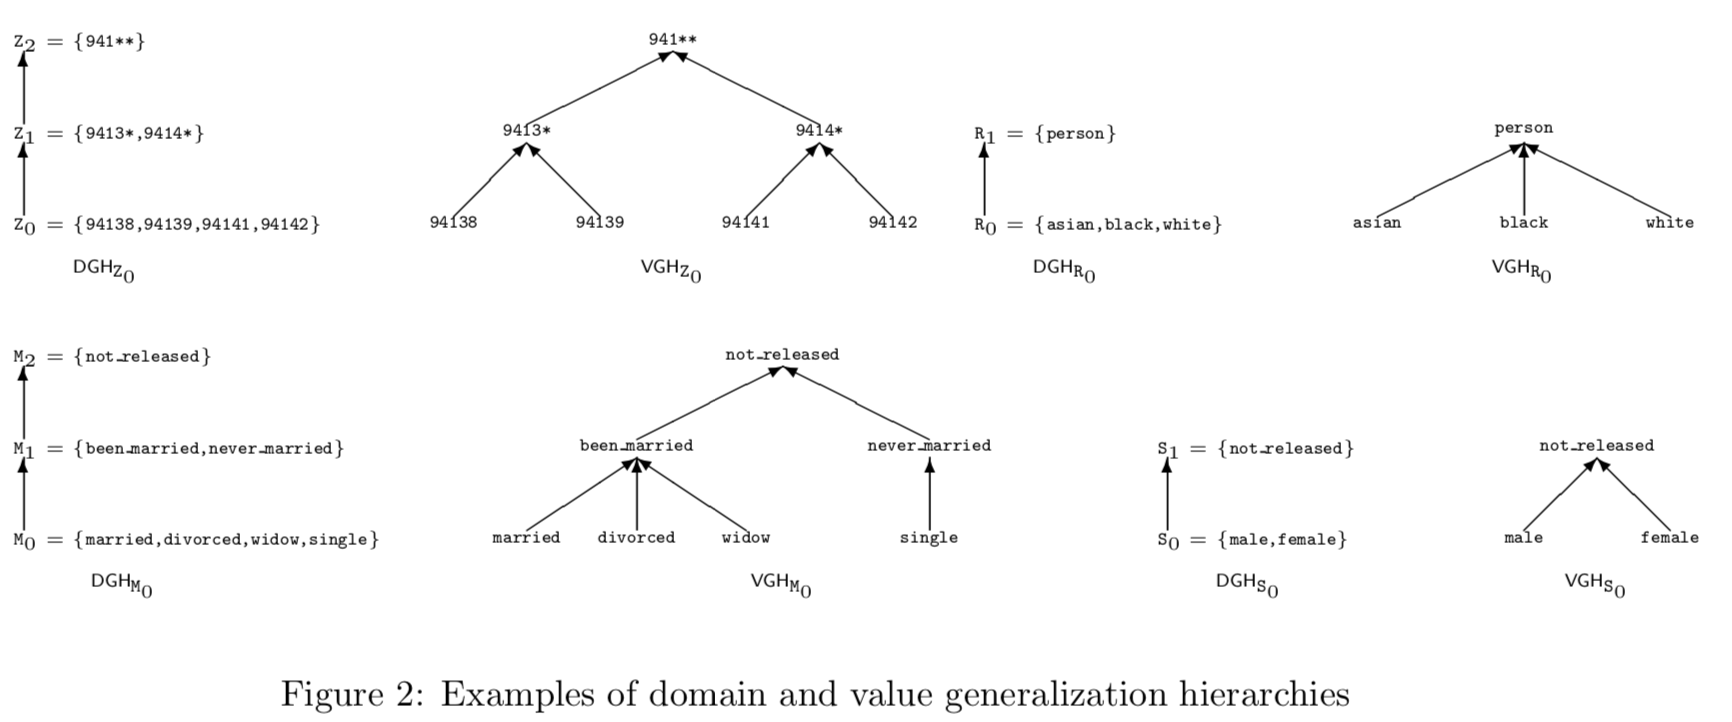
\includegraphics[width=0.95\textwidth]{../images/dgh-vgh.png}
	\caption{}
	\label{dgh-vgh}
\end{figure}
\paragraph{DGH的格表示} 给定一个域元组$DT=<D_1,...,D_n>$,我们可以定义关于DT的域泛化结构为$DGH_{DT}=DGH_{D_1} \times ... \times DGH_{D_n}$,即DT的DGH是其每个元素的DGH的笛卡尔积。由于每个$DGH_{D_i}$都是全序的,因此$DGH_{DT}$是一个关于DT的格(lattice),其最小值(DT)在底部,最大值在顶部。如图 \ref{dgh-lattice}所示。
\begin{figure}[H]
	\centering
	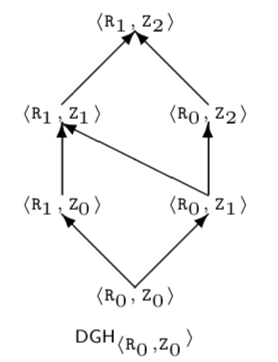
\includegraphics[width=0.3\textwidth]{../images/dgh-lattice.png}
	\caption{DGH的格表示}
	\label{dgh-lattice}
\end{figure}

\paragraph{泛化策略(generalization strategy)} $DGH_{DT}$格中的一组边及其节点组成的集合成为泛化策略。如图 \ref{generalization-strategy} 所示。
\begin{figure}[H]
	\centering
	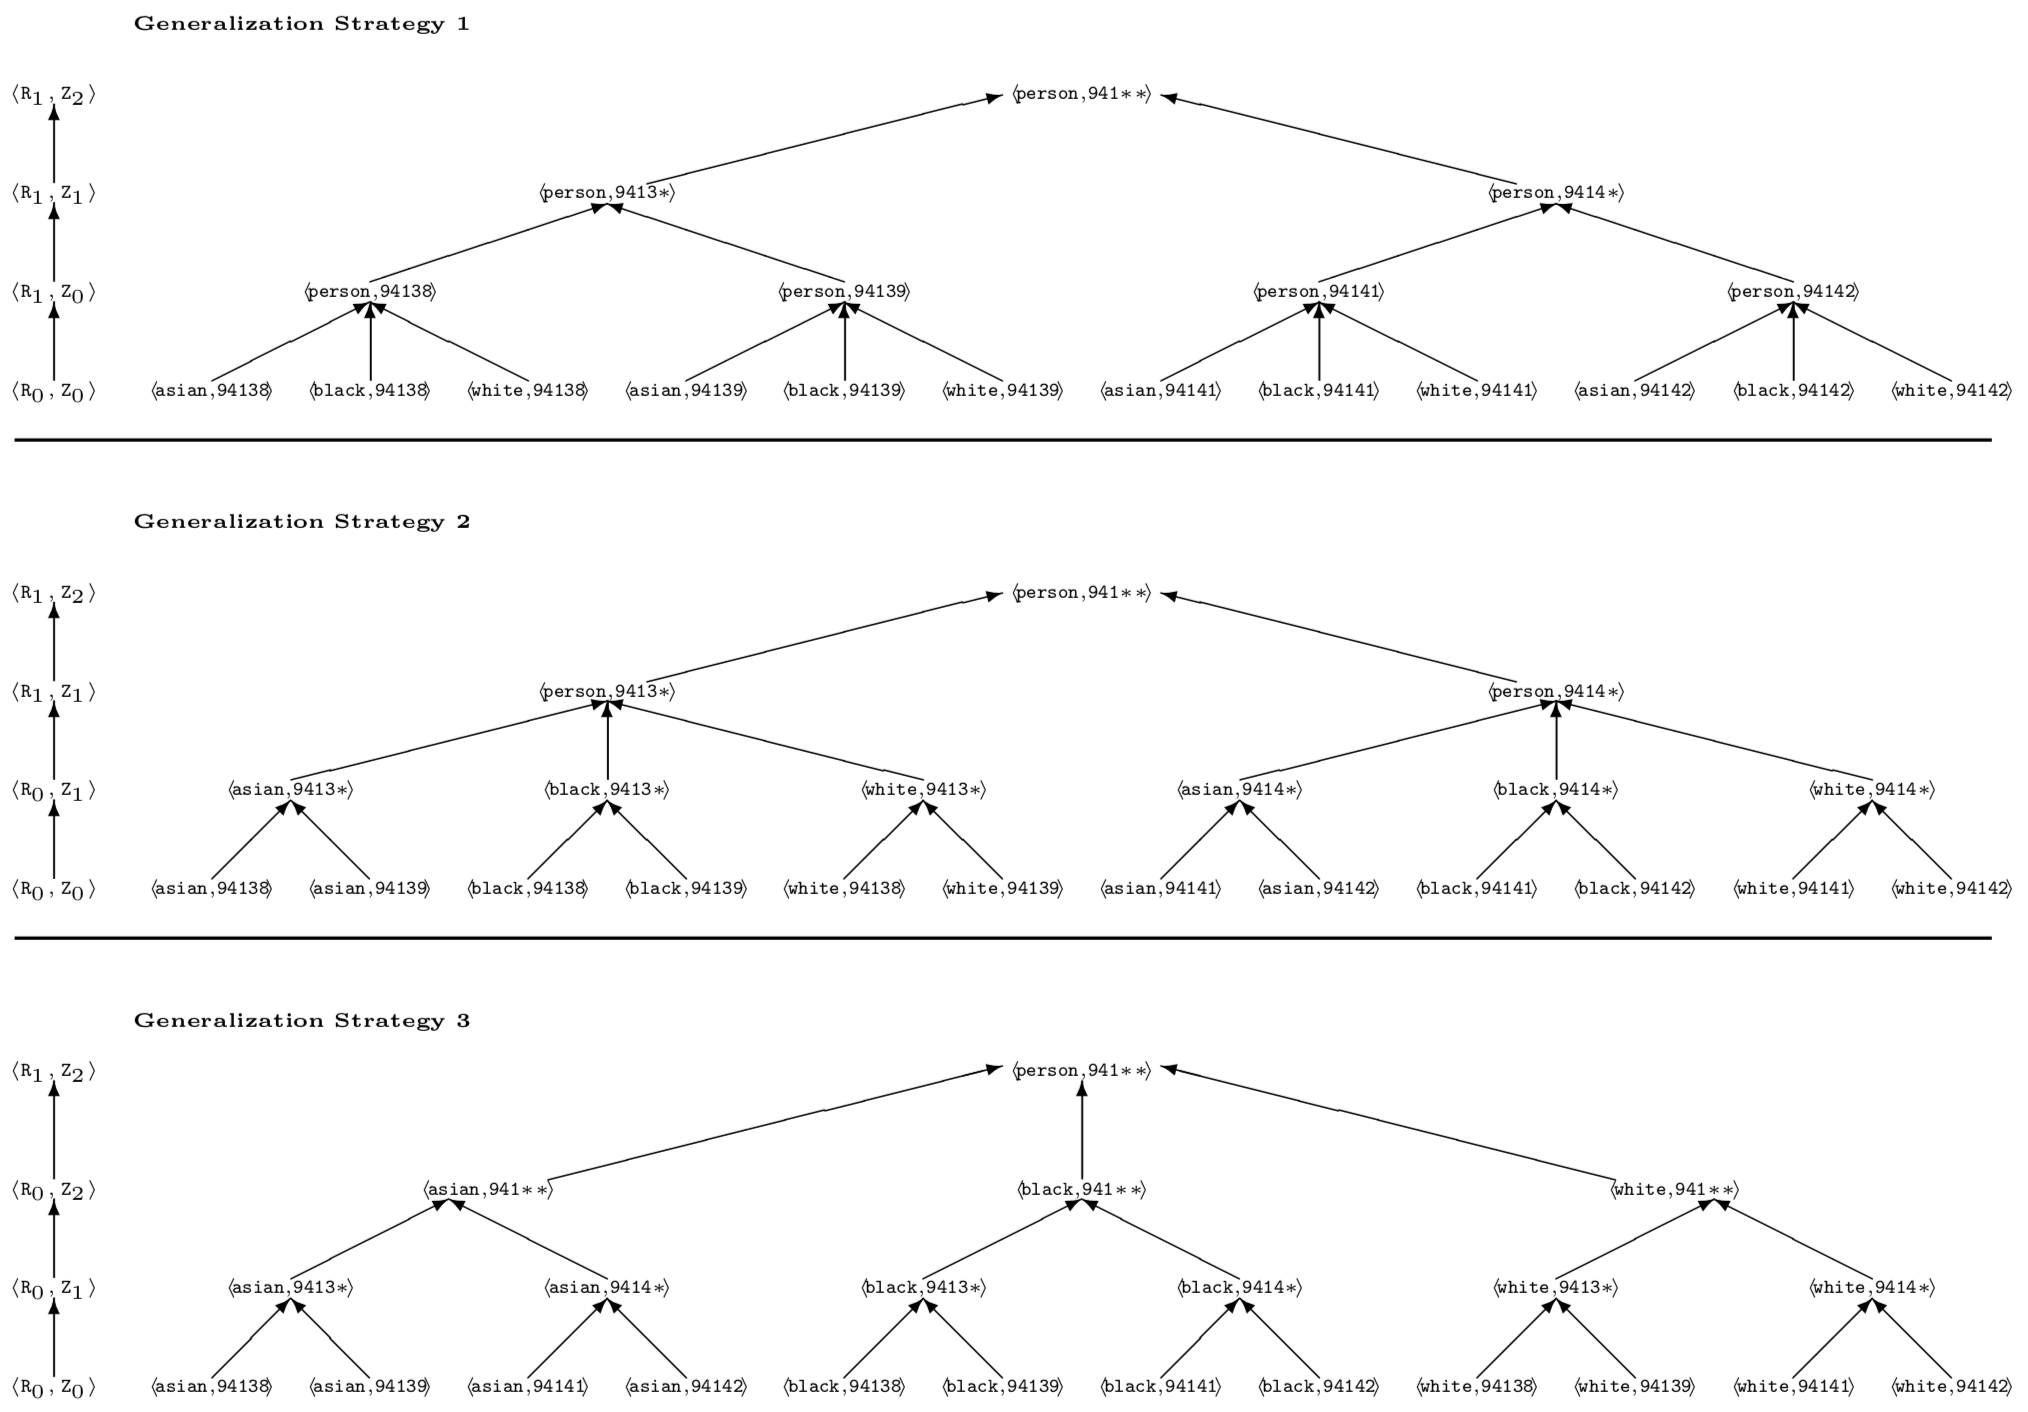
\includegraphics[width=1\textwidth]{../images/generalization-strategy.png}
	\caption{DGH的格表示}
	\label{generalization-strategy}
\end{figure}

\subsubsection{Generalized table and minimal generalization}
\paragraph{属性的值域} 定义$dom(A_i,T)$表示属性$A_i$在T中的值域。
\paragraph{泛化表(Generalized Table)} 令$T_i(A_1,...,A_n)$和$T_j(A_1,...,A_n)$是具有相同属性(字段)的两个表,若满足以下条件则称$T_j$是$T_i$的泛化,记作$T_i \preceq T_j$:
\begin{itemize}
	\item $|T_i| = |T_j|$(两个表中的数据量一致)
	\item $\forall A_z \in \left \{ A_1,...,A_n \right \}: dom(A_z, T_i) \leq dom(A_z, T_j)$ (每个属性满足一致的域泛化关系)
	\item 每个属性值满足一致的值泛化关系
\end{itemize}
\paragraph{距离向量(distance vector)} 两个表$T_i$、$T_j$满足$T_i \preceq T_j$,从$T_i$到$T_j$的距离向量记作$DV_{i,j}=[d_1,...,d_n]$,其中$d_z$是$DGH_{D_z}$中$D_i$到$D_j$的距离。
\paragraph{距离向量的偏序关系} 两个距离向量$DV$、$DV'$,如果所有的$d_i \leq d_i'$,则有$DV \leq DV'$。因此,域泛化结构可以看做是距离向量的格,如图 \ref{lattice-on-dv} 所示。
\begin{figure}[H]
	\centering
	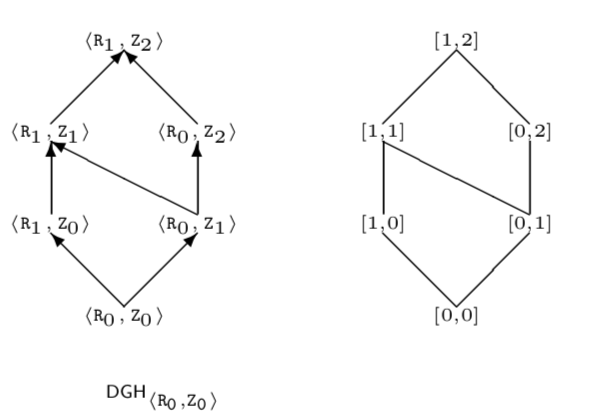
\includegraphics[width=0.5\textwidth]{../images/lattice-on-dv.png}
	\caption{DGH的距离向量格表示}
	\label{lattice-on-dv}
\end{figure}

\paragraph{k-minimal 泛化(generalization)} 两个表$T_i$、$T_j$满足$T_i \preceq T_j$,如果$T_j$满足下列两个条件就称$T_j$是$T_i$的一个k-minimal泛化:
\begin{itemize}
	\item $T_j$满足k-anonymity
	\item $\forall T_z: T_i \preceq T_z satisfies k-anonymity \Rightarrow \neg (DV_{i,z} \leq DV_{i,j})$(不存在任何一个比$T_j$小,而且满足k-anonymity的泛化表)。
\end{itemize}

\subsection{Suppressing data}
\paragraph{} 泛化的好处是可以在满足k-anonymity的条件下发布表中所有的数据条目,而suppression则通过移除某些条目来满足k-anonymity,同时减少泛化所需的步骤。

\paragraph{带suppression的泛化表(generalized table with suppression)} 与泛化表相比,它不要求$|T_i| = |T_j|$,而是要求$|T_i| \geq |T_j|$,也就是说,泛化表的条目可以比原表少。

\paragraph{最小要求抑制(minimal required suppression)} $T_j$是$T_i$的满足k-anonymity的泛化,满足下列条件时,我们称对$T_j$执行了最小要求抑制(也就是说,$T_j$是满足k-anonymity的抑制中条目最多的):
\begin{equation}
	iff \enspace \forall T_z: T_i \preceq T_j, DV_{i,z} = DV_{i,j}, T_z \enspace satisfies \enspace k-anonymity \Rightarrow |T_j| \geq |T_z|.
\end{equation}


\paragraph{} 对任意一个表,若想要它满足k-anonymity,最简单的办法是移除QI重复次数少于k的数据条目。这样并不是好的做法,我们最希望得到的是一个执行了最小要求抑制的泛化结果,尽可能保留数据条目。泛化和抑制应当交叉使用,而问题是:以损失数据进度为代价的泛化和以损失数据完整性为代价的抑制,哪种更好。

\paragraph{} 我们假设一个可接受的抑制值MaxSup,当被移除的数据条目少于它时,我们认为这是可接受的,也就是说,此时抑制比泛化更好。这是由于抑制只影响一条数据,而泛化影响整个数据表的某个属性。


\paragraph{带suppresion 的k-minimal泛化}  两个表$T_i$、$T_j$,满足$T_i \preceq T_j$,若满足以下条件则称$T_j$是$T_i$的k-minimal泛化:
\begin{itemize}
	\item $T_j$ 满足执行最小要求抑制的k-anonymity。
	\item $ |T_i| - |T_j| \leq MaxSup$.(不需要执行比要求的更多的抑制操作)
	\item $\forall T_z: T_i \preceq T_z$ and satisfies conditions 1 and 2 $ \Rightarrow \neg (DV_{i,z} < DV_{i,j})$ (不存在满足以上条件,且比它DV更小的泛化)。
\end{itemize}

\subsection{Computing a k-minimal generalization}
\paragraph{定理5.1} 表$T_i = PT[QI]$,DT是其值域元组,$T_i$的每一个k最小泛化都是$DGH_{DT}$中的泛化策略的局部最小泛化。
\paragraph{} 由定理5.1可知,可以这样计算一个k最小泛化:遍历每一个泛化策略,沿着DT到DGH的最大值的方向出发,直到找到一个泛化结果,是的其满足k-anonymity和抑制阈值为止。给定$D_i$由DT到DGH的顶部的高度为$h_i$,DT在DGH中的不同策略的数量为$\frac{(h_i+...+h_n)!}{h_1!...h_n!}$。
\paragraph{定理 5.2} 表$T_i = PT[QI]$,$T_j$、$T_z$是它的两个满足最小要求抑制的泛化,则有:$DV_{i,j} < DV_{i,z} \Rightarrow |T_j| \leq |T_z|$。直观来看,由于$T_z$更加“泛化”,它要满足抑制要求就只需要移除更少的条目。
\paragraph{推理 5.1} 由定理5.1可知,$|T_j| \leq |T_z| \Rightarrow (|T_i| - |T_j|) \geq (|T_i| - |T_z|)$,则:$|T_i| - |T_j| \leq MaxSup \Rightarrow |T_i| - |T_z| \leq MaxSup$,反之,$|T_i| - |T_z| > MaxSup \Rightarrow |T_i| - |T_j| > MaxSup$。因此,如果一个具有$DV_{i,z}$的表$T_z$不能在抑制阈值MaxSup范围内提供k-anonymity,则所有具有$DV_{i,j}<DV_{i,z}$的表$T_j$也不能。
\paragraph{DV的高度} 定义为在一个DV格VL中,从结点DV到格VL最小元素的距离。表示为$height(DV,VL)$。
\paragraph{引理 5.1} 格$VL=<DV, \leq >$,$\forall DV_{i,j}, DV_{i,z} \in DV$,有:$DV_{i,j} < DV_{i,z} \Rightarrow height(DV_{i,j},VL) < height(DV_{i,j}, VL)$。

\paragraph{} 通过以上引理,可以推理出实现k-anonymity的策略。设$\top$是VL的最大值,对每一个高度h,如果在高度h对应的DV不满足指定的泛化,那么任何小于高度h的DV都不满足指定的泛化。因此,我们可以通过二分搜索的方法找到满足指定泛化的最小高度h,并找到相应的DV。假设$h=height(\top,VL)$,我们首先评估高度$\left \lfloor \frac{h}{2} \right \rfloor$处的所有DV是否满足指定的泛化,如果满足,则记录下这些DV,然后在小于$\left \lfloor \frac{h}{2} \right \rfloor$高度处递归寻找是否有满足指定泛化的更小的DV。反之,则在大于$\left \lfloor \frac{h}{2} \right \rfloor$高度处寻找。此过程类似二分查找。
\paragraph{} 此算法基于预定义的DGH,采用二分法查找DV。
















\section{l-Diversity: Privacy Beyond k-Anonymity\cite{l-diversity} }

\subsection{Introduction}
\subsubsection{k-anonymity面临的两种形式的攻击}
\paragraph{} k-anonymity面临两种形式的攻击:
	\subparagraph{同质化攻击(Homogeneity attack)} 如同前面所提的的“互补发布攻击”、“时间攻击”,由于数据发布时,并不是所有字段都是QI,而同一组QI的值相同的数据中,会出现敏感字段都相同的情况,而且这种情况并不罕见。在这种情况下,如果数据集仅执行k-anonymity,则会由于敏感字段缺乏多样性而使得攻击者可以重新识别数据集个体,从而造成信息纰漏。同质化攻击问题的一种解决方案就是本文所讲的l-diversity模型。
	\subparagraph{背景知识攻击(Background knowledge attack)} 就算数据由于多样性的存在而不会受到同质攻击,但也有可能会由于背景知识(例如,可以从日常生活看出某人肯定不会患有某种特定疾病)的存在而是多样性容易排除,从而使得敏感信息泄露。
	
\subsection{定义}
\paragraph{数据泛化(Data generalization)} 将一个数据集进行分组,各个分组之间互不重叠。其形式化定义为:域$D^*=\left \{P_1,P_2,...\right \}$是域D的泛化,如果$\cup P_i = D$ and $P_i \cap P_j = \O, i \neq j $。$\phi_{D^*}(x)$表示$D^*$包含x的元素P。

\paragraph{攻击者(Adversary)的背景知识} 攻击者可能知道以下几类背景知识:
	\subparagraph{} 攻击者可能知道已发布的表T的泛化$T^*$,也就是说,知道T的属性的值域。
	\subparagraph{} 攻击者可能知道某些个体存在于表中。
	\subparagraph{统计(demographic)背景知识} 攻击者可以知道表中字段的值的分布。

\subsection{贝叶斯优化隐私模型(Bayes-Optimal Privacy, BOP)}
\paragraph{两个假设} 为简化模型,给出两个假设:
\begin{itemize}
	\item 数据表T是全集的一个随机样本集;
	\item 个体只有一个敏感字段。
\end{itemize}
另外,还假设一个比较糟糕的情况:攻击者知道准标识符Q和敏感字段S的联合分布。
\paragraph{度量} 我们用两个指标对隐私纰漏进行度量:
	\subparagraph{先验置信(prior belief)} 已知目标个体t的准标识符的值q的情况下,其敏感字段值为s的概率:
	\begin{equation}
		\alpha_{(q,s)} = P_f(t[S]=s|t[Q]=q)
	\end{equation}

	\subparagraph{后验置信(posterior belief)} 已知目标个体t的准标识符的值q,以及其泛化$t^*$的情况下,其敏感字段值为s的概率:
	\begin{equation}
		\beta_{(q,s,T^*)}=P_f(t[S]=s|t[Q]=q \wedge \exists t^* \in T^*, t \overset{*}{\rightarrow}t^* )
	\end{equation}
\paragraph{定理3.1} 令$n_{q^*,s'}$是表中出现$(q^*, s')$对的个数。

\paragraph{定理3.1的证明}

\subsubsection{隐私原则}
\paragraph{数据表发布后可能泄露隐私的两种方式}
	\subparagraph{正纰漏(Positive Disclosure)} 如果发布数据表后,可以提升攻击者正确识别目标的概率,例如,对于一个q,其对应的s的值都是同一个(同质化攻击),那就是正纰漏。 
	\subparagraph{负纰漏(Negative Disclosure)} 如果发布数据表后,攻击者可以从中排除一些关于目标的错误的敏感值,例如,根据背景知识可以排除特定个体的一些敏感值,那就是负纰漏。
\paragraph{不提供信息原则(Uninformative Principl)} 隐私的理想定义应该满足不提供信息原则,即:表的发布并不能为攻击者带来除了背景信息以外的其他信息。此原则有很多实例化的方式,他们都属于贝叶斯优化隐私定义。其中一个是:
	\subparagraph{$(\rho_1, \rho_2)-Private$} 给定表$T^*$和两个常数$\rho_1,\rho_2$。如果$\alpha_{(q,s)} < \rho_1 \wedge \beta_{(q,s,T^*)} > \rho_2$,或者$\alpha_{(q,s)} < 1 - \rho_1 \wedge \beta_{(q,s,T^*)} > 1 - \rho_2$,我们就说发生了“$(\rho_1, \rho_2)$-privacy breach”。如果$(\rho_1, \rho_2)$-privacy breach没有发生,我们就说表$T^*$满足$(\rho_1, \rho_2)-Private$。

\subsubsection{BOP的局限}
	
\paragraph{} BOP存在着一些缺陷,使其无法在实践中使用。包括:
	\subparagraph{不充分知识} 数据发布者不可能完全知道数据的分布。
	\subparagraph{对攻击者的无知} 数据发布者不知道攻击者到底知道什么。
	\subparagraph{实例知识} 理论定义不能定义那些无法被概率模型建模的知识。例如,Bob的儿子可能会告诉Alice,Bob没有糖尿病。
	\subparagraph{多攻击者} 可能会有多个不同知识水平的攻击者存在,他们具有的背景知识都不同,数据发布者都必须考虑到。
	
\subsection{l-diversity: 一种实用的隐私定义}
\paragraph{} l-diversity可以克服上述的BOP实践中存在的问题。

\subsubsection{l-diversity 原则}
\paragraph{等价类($q^*-block$)} 表$T^*$中的一组数据,他们的非敏感值都被泛化为$q^*$。
\paragraph{l-diversity原则} 如果有一个$q^*-block$,它的隐私属性S包含至少$l$个良表示(well-represented)值,我们就说这个$q^*-block$是$l-diverse$的,如果表中所有的$q^*-block$都是$l-diverse$的,那么这个表就是$l-diverse$的。
\paragraph{} 此原则主张确保每一个$q^*-block$的敏感字段具有至少l个良表示值,但并没有说明良表示意味着什么。最简单的,我们可以将“l个良表示值”理解为“l个不同的值”。另外,定义不同的良表示值也可以得到不同的实例。
\subsubsection{l-diversity的实例}
\paragraph{} 根据不同的良表示定义,可以得到不同的l-diversity定义。包括:可区分l-diversity、熵l-diversity、递归l-diversity等。

\paragraph{Distinct(可区分) l-diversity} 要求每个等价类中至少有l个可区分的值。它存在一个缺陷:如果某一个取值的频率明显高于其他取值,这将使得观察者可以以较高的置信度认为这一等价类中的敏感属性都取这个值。

\paragraph{Entropy l-diversity} 设$p_(q^*,s)$为等价类中敏感值为s的概率,那么表满足l-diversity的条件是,每一个等价类都满足:
\begin{equation}
	- \Sigma_{s \in S} p_(q^*,s) \log(p_(q^*,s)) \geq \log(l)
\end{equation}
这要求整个表的熵至少是$\log(l)$,也就是要求至少有l个可区分的值。这并不容易实现,特别是当某个敏感值非常常见的时候。

\paragraph{Recursive(c,l)-diversity} 递归l-diversity。 

\subsubsection{多敏感属性的情形}
\paragraph{} 以上讨论都基于一个基本的假设:每条数据只有一个敏感字段。
\paragraph{Multi-Attribute l-diversity} 若把$S_i$之外的所有S都当做Q还满足l-diversity,那么表T就满足l-diversity。

\bibliographystyle{ieeepes}
\bibliography{../Saliency}
\end{document}



























































